
\subsection{Dataset and Evaluation Method}
The dataset we used in our experiments is provided by StackOverflow.com. Currently, there are 2.2 million questions, 4.8 millions answers, over 35 thousands tags in this dataset\cite{DataDump}.

We prepared 1,050,000 posts(a post is either a question or an answer)  as the training data $S_{train}$, and randomly sampled 500 posts along the timeline as our test dataset $S_{test}$.

We use the the precision and recall as the metrics to evaluation the classification methods.
$$ \text{Precision}=\frac{tp}{tp+fp} $$
$$ \text{Recall}=\frac{tp}{tp+fn} $$
where $tp$ is the count of true positive, $fp$ the false positive and $fn$ the false negative.

\subsection{Experimental Results}
\subsubsection{Naive Bayes}
In naive bayes, we choose the top-rank $N$ tags as our predicted tags. Figure \ref{fig:naive} shows the precision/recall of bayes classifier with different $N$. We can see that the recall increases as $N$ goes up; whereas the precision drops when $N$ increases.

\begin{figure}[htb!]
\centering%
    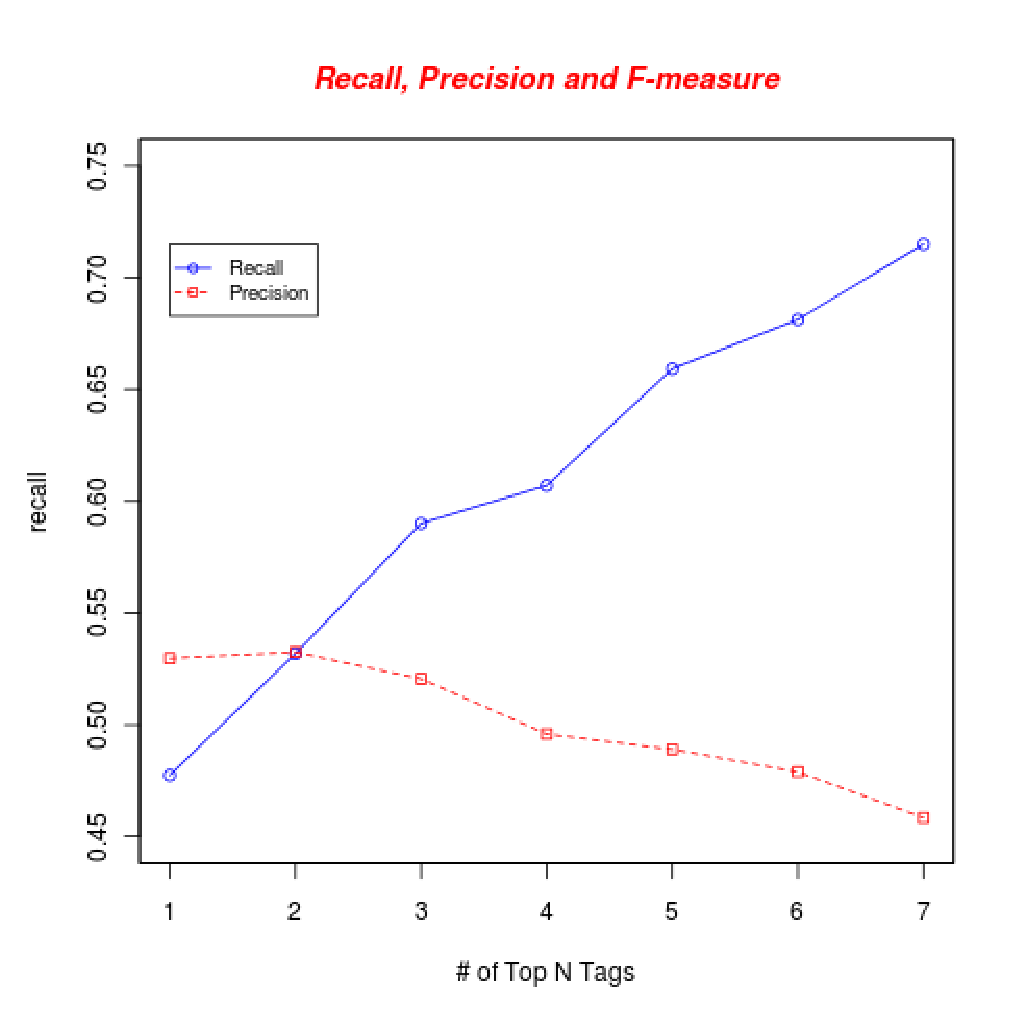
\includegraphics[scale=0.5]{naives.eps}
\caption{Tag Prediction By Naive Bayes}
\label{fig:naive}
\end{figure}]


\subsubsection{Logistic Regression}
Under Construction

\subsubsection{SVM}
Under Construction

\subsection{Comparison and Conclusion}
Under Construction. This part depends on the experimental results of all the three models.
